
An RFID system is composed of three components:
\begin{itemize}
    \item A transponder (tag), consists of antenna, chip, and sometimes a battery. It is the data-carrying device.
    \item An interrogator (the reader/write device), consists of reader antenna, radio-frequency electronics, and control module
    \item A controller (host electronic or computer), consists of database 
\end{itemize}


\begin{figure}[htp]
    \centering
    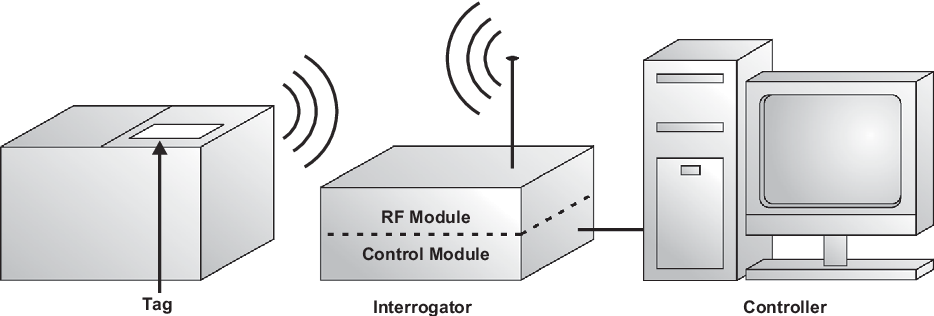
\includegraphics[scale=0.45]{Figs/RFID_Blocks.png}
    \caption{The basic components to an RFID system. \cite{laran2004basic}}
    \label{fig:RFIDBlocks}
\end{figure}


Some RFID systems can have the interrogator and the controller be one component. The simple interaction between these components is that the tag and interrogator communicate information between each other via radio-frequency (RF) waves. This interaction occurs when the tagged specimen enters the read zone of the interrogator, retrieves information from the tag. The information that tags can store can be serial numbers, time stamps,  or other useful data. Once the interrogator retrieves the tag's information the controller can implement another procedure such as recording inventory, granting access, active another electronic such as a motor, etc. 

The RFID tags fall into two categories, passive and active transponders. Passive RFID tags do not have on-board power supply instead they obtain their power from the interrogator's transmitted signal (magnetic or electromagnetic field). The tag transmits its data via modulation (e.g. by load modulation or modulated back-scatter). In most cases, passive tags are smaller and less expensive than active tags. Active tags contain an on-board power supply, such as a battery or solar cell, to provide voltage to the chip. The active tags can generate their own fields and modulation thus increasing the read-range between the transponder and the interrogator. Important to note that active tags are typically not able to generate high-frequency signals alone, can only modulate the fields from the interrogator.    
Tags can also be categorized as read-only (RO) and read/write (RW). The RO tags can only be read. Once these RO tags are fabricated their data can be altered. Typically used for static information such as part numbers, ID, serial numbers, etc. The RW provides more flexibility such as allowing the data to be changed, storing much more information than RO tags, and easy accessibility.   

